\documentclass[a4paper,11pt]{article}
\usepackage{physics}
\usepackage{amsmath}
\numberwithin{equation}{section}
\usepackage{siunitx}
\usepackage{braket}
\usepackage{authblk}
\usepackage[a4paper, margin=1.5in]{geometry}
\usepackage{parskip}
\setlength{\parindent}{15pt}
\usepackage{tikz}
\usetikzlibrary{arrows, calc, patterns, angles, quotes}
\usetikzlibrary{decorations.pathmorphing}
\usepackage{amssymb}
\usetikzlibrary{shapes.geometric}
\usepackage[section]{placeins}
\usepackage{pgfplots}
\usepackage{clock}
\usepackage[clock]{ifsym}
\usetikzlibrary{shapes}
\usepackage{amsthm}
\theoremstyle{definition}
\newtheorem{defn}{Definition}[section]
\newtheorem{prop}{Proposition}[section]
\newtheorem{propty}{Properties}[section]
\newtheorem{rmk}{Remark}[section]
\newtheorem{exmp}{Example}[section]
\newtheorem*{prob*}{Problem}
\newtheorem{prob}{Problem}[section]
\newtheorem*{sln*}{Solution}
\newtheorem{sln}{Solution}[section]
\usepackage{empheq}
\usepackage{hyperref}
\usepackage{tensor}
\usepackage{xcolor}
\hypersetup{
	colorlinks,
	linkcolor={black!50!black},
	citecolor={blue!50!black},
	urlcolor={blue!80!black}
}
\newcommand{\p}{\partial}
\newcommand{\lag}{\mathcal{L}}


%\usepgfplotslibrary{external}
%\tikzexternalize

\begin{document}
\begin{titlepage}\centering
 \clearpage
 \title{\textsc{\bf{CLASSICAL FIELD THEORY}}\\\smallskip A Quick Guide\\}
 \author{\bigskip Huan Q. Bui}
 \affil{Colby College\\Physics \& Statistics \\Class of 2021\\}
 \date{\today}
 \maketitle
 \thispagestyle{empty}
\end{titlepage}

\newpage

\section*{Preface}
\addcontentsline{toc}{subsection}{Preface}

Greetings,\\

\textit{Classical Field Theory, A Quick Guide to} is compiled based on my independent study PH492: Topics in Classical Field Theory notes with professor Robert Bluhm. Sean Carroll's \textit{Spacetime and Geometry: An Introduction to General Relativity}, along with other resources, serves as the main guiding text. This text also references a number of other texts such as \textit{Quantum Field Theory} by Ryder, \textit{Quantum Field Theory} by Mandl and Shaw, \textit{Gauge Theories Of The Strong, Weak, And Electromagnetic Interactions} by Quigg.   \\

This text is a continuation of \textit{General Relativity and Cosmology, A Quick Guide to}. Familiarity with classical mechanics, linear algebra, vector calculus, and especially general relativity is expected. There will be a quick review of general relativity where important concepts are revisited and important derivations highlighted, but familiarity with basic notions such as geodesics, Christoffel symbols, the Riemann curvature tensors, etc. is assumed. \\ 

Enjoy!


\newpage

\tableofcontents

\newpage

\section{Introduction to Classical Field Theory}
\newpage
\section{Group Theory: a quick guide in a quick guide}
\begin{enumerate}
	\item Consider an N-dimensional vector with complex elements. A gauge transformation that takes $\vert z\vert^2 \to \vert z \vert^2$ (modulus preserving) is call a U(N) gauge transformation. The letter ``U'' denotes ``unitary.'' These kinds of transformations can be represented by a unitary matrix, which is defined as a matrix whose conjugate transpose is the same as its inverse. If $z\to Uz$, then 
	\begin{align*}
	\vert z\vert^2 \to (Uz)^\dagger(Uz) = z^\dagger U^\dagger U z =z^\dagger z =\vert z\vert^2,
	\end{align*} 
	hence modulus preserving.\\
	
	Note that the transformation $e^{i\alpha}$ is unitary. It is simply a 1$\times$1 unitary matrix. This immediately implies that complex scalars have a U(1) gauge invariance.\\
	
	The special group of U(N) transformations is denoted SU(N), which represents those with $\det U= 1$. 
	\item Consider another N-dimensional real-valued-element vector. We denote the group of orthogonal transformations O(N). Orthogonal transformations are orthogonal, i.e., length-preserving. 
	\begin{align*}
	(Ox)^\top(Ox) = x^\top O^\top O x = x^\top x = \vec{x}^2
	\end{align*} 
	Once again, we denote the special group of the O(N) the SO(N) group. This group represents transformations with $\det O = 1$. The Lorentz group is a sub-group of SO(N), as the norm is defined differently, nevertheless it is still length-preserving. We call the Lorentz group SO(3,1), signifying that one sign is different from the other three. 
\end{enumerate}

\newpage
\section{Introduction to the Lagrangian and the Principle of Least Action}
\begin{prop}
	All fundamental physics obeys least action principles.
\end{prop}
The action $S$ is defined as
\begin{align*}
S = \int_{a}^{b}\mathcal{L}\,dt.
\end{align*}
where $\mathcal{L}$ is called the Lagrangian.\\

Refer for Farlow's \textit{Partial Differential Equation}, page 353, for detailed explanation of Lagrange's calculus of variations.\\

I will derive the Euler-Lagrange equation(s) here, but we are not going to use it in the following subsection for the introduction to field theory for now. \\
\begin{align*}
\frac{\partial \mathcal{L}}{\partial \phi} - \partial_\mu\frac{\partial \mathcal{L}}{\partial(\partial_\mu \phi)} = 0.
\end{align*}
\subsection{A Classical-Mechanical Example}
In this subsection we take a look at how the Lagrangian formulation of classical mechanics can give rise to Newton's second law of motion. In mechanics, the Lagrangian often takes the form:
\begin{align}
\mathcal{L} = K - V,
\end{align}
where $K$ is the kinetic energy, and $V$ is the potential energy. Let us consider a simple example where
\begin{align*}
K &= \frac{1}{2}m\dot{x}^2\\
V &= V(x).
\end{align*}
Variations on the Lagrangian gives
\begin{align*}
\delta \mathcal{L} &= \delta\left( \frac{1}{2}m\dot{x}^2 - V(x) \right)\\
&= m\dot{x}\delta \dot{x} - \frac{dV}{dx}\delta x\\
&= m\dot{x}\dot{\delta x} - \frac{dV}{dx}\delta x\\
&= m \left( -\ddot{x}\delta x + \frac{d}{dt}\dot{x}\delta x \right) - \frac{dV}{dx}\delta x\\
&= -m\ddot{x}\delta x - m\frac{d}{dt}\dot{x}\delta x - \frac{dV}{dx}\delta x. 
\end{align*}
It follows that the variations on the action gives
\begin{align*}
\delta S = \int_{a}^{b}\delta L \,dt = -\int_a^b\left( m\ddot{x} + \frac{dV}{dx} \right)\delta x\,dt.
\end{align*}
The principle of least action requires $\delta S = 0$ for all $\delta x$. Therefore it follows that
\begin{align*}
m\ddot{x} + \frac{dV}{dx} = 0,
\end{align*}
which is simply Newton's second law of motion in disguise. \\

Before we move on, we should note that in order for the Lagrangian formulation to work in electromagnetism or in general relativity, we need to promote the Lagrangian to its relativistic version where the Lagrangian is given by
\begin{align*}
L = \int_a^b\mathcal{L}\,d^3x.
\end{align*}
$\mathcal{L}$ is called the Lagrangian density, but we can colloquially refer to it as ``the Lagrangian.'' The relativistic action hence takes the form
\begin{align*}
S = \int \mathcal{L}\,d^4x,
\end{align*}
where $d^4x$ implies integrating over all spacetime.

\subsection{Introduction to Fields}
In field theory, most physical objects are described as ``fields.'' Let us dive into the first two fields that we are more or less familiar with: scalar fields and vector fields. 

\newpage
\section{Gauge Invariance}
\subsection{Introduction}
From studying Maxwell's equations, we know that there is more than one way to choose a vector potential $A_\mu$ that describes the same electromagnetic field. This freedom is called \textit{gauge invariance}. We will explore the idea of gauge invariance  in the context of a continuous symmetry of the Lagrangian, which leads to the conservation of electric charge and other important consequences under Noether's theorem.\\

In the subsequent subsections, we will explore and try to understand the idea of gauge invariance. We will start out with gauge invariance in classical electrodynamics. Then, we will look briefly at phase invariance in quantum mechanics and ultimately field theory.  
\subsection{Gauge Invariance in Classical Electrodynamics}
Recall the second of Maxwell's equations, written in differential form:
\begin{align*}
\div{\mathbf{B}} = 0.
\end{align*}
Following from a vector calculus identity, this means the magnetic field can be expressed as a curl of some vector potential, called $\mathbf{A}$:
\begin{align*}
\div{\mathbf{B}} = \div{\curl\mathbf{A}} = 0.
\end{align*}
Now, we also know that the curl of a conservative vector field is zero, it is also true that
\begin{align*}
\curl{(\mathbf{A} + \grad{\Lambda})}= \curl{\mathbf{A}} + \curl{\grad{\Lambda}} = \curl{\mathbf{A}}.
\end{align*}
It follows that this new vector potential $\mathbf{A} + \grad{\Lambda}$ also describes the same magnetic field $\mathbf{B}$:
\begin{align*}
\mathbf{B} = \curl{(\mathbf{A} + \grad{\Lambda})} = \curl{\mathbf{A}}.
\end{align*}

Next, consider Faraday-Lenz law:
\begin{align*}
\curl{\mathbf{E}} = -\frac{\p \mathbf{B}}{\p t}.
\end{align*}
Since $\mathbf{B} = \curl{\mathbf{A}}$, this can be re-written as:
\begin{align*}
\curl{\left(\mathbf{E} + \frac{\p \mathbf{A}}{\p t}\right)} = 0.
\end{align*}
This suggests that 
\begin{align*}
\mathbf{E} + \frac{\p \mathbf{A}}{\p t} 
\end{align*}
is some conservative vector field, which we shall identity as $-\grad{V}$, where $V$ is the scalar potential:
\begin{align*}
\mathbf{E} + \frac{\p \mathbf{A}}{\p t}  = -\grad{V}.
\end{align*}
Now, in order for the electric field $\mathbf{E}$ to remain invariant under the transformation
\begin{align*}
\mathbf{A} \to \mathbf{A} + \grad{\Lambda},
\end{align*}
we must require that
\begin{align*}
\mathbf{E'} &= \mathbf{E}\\
-\grad{V'} - \frac{\p \mathbf{A'}}{\p t} &= -\grad{V} - \frac{\p \mathbf{A}}{\p t}\\
-\grad{V'} - \frac{\p }{\p t}\left( \mathbf{A} + \grad{\Lambda} \right) &= -\grad{V} - \frac{\p \mathbf{A}}{\p t}\\
\grad{V'} &= \grad{V} + \frac{\p }{\p t}\grad{\Lambda}\\
\grad{V'} &= \grad{V} + \grad{\left( \frac{\p \Lambda}{\p t}\right)},
\end{align*}
i.e,
\begin{align*}
V' = V + \frac{\p \Lambda}{\p t}.
\end{align*}
So, the scalar potential has to undergo the transformation
\begin{align*}
V \to V + \frac{\p \Lambda}{\p t}.
\end{align*}

Now, if we define the 4-vector potential as
\begin{align*}
A^\mu = (V,\mathbf{A}),
\end{align*}
then everything we have done so far can be encoded in the 4-curl of $A^\mu$, which we define as the anti-symmetric electromagnetic field strength tensor
\begin{align*}
F^{\mu\nu} = -F^{\nu\mu} = \p^\mu A^\nu - \p^\nu A^\mu = \begin{pmatrix}
0 & -E_1 & -E_2 & -E_3\\
E_1 & 0 & -B_3 & B_2\\
E_2 & B_3 & 0 & -B_1\\
E_3 & -B_2 & B_1 & 0
\end{pmatrix}.
\end{align*}
We can verify that $F^{\mu\nu}$ is invariant under the transformation
\begin{align*}
A^\mu \to A^\mu - \p^\mu\Lambda
\end{align*}
or
\begin{align*}
A_\mu \to A_\mu + \p_\mu \Lambda,
\end{align*}
where $\Lambda(x)$ is an arbitrary scalar field of the coordinate. The fact that many different four-vector potentials yield the same electromagnetic fields, and thus describe the same physics, is a manifestation of the gauge invariance of classical electrodynamics.\\

From \textit{General Relativity \& Cosmology, A Quick Guide to...}, we have verified how the Maxwell's equations in covariant notation:
\begin{align*}
\p_\mu F^{\mu\nu} &= -J^\nu\\
\p_\sigma F_{\mu\nu} + \p_\mu F_{\nu\sigma} + \p_\nu F_{\sigma\mu} &= 0
\end{align*} 
where the \textit{4-current} $J^\nu$ is defined as
\begin{align*}
J^\nu = (\p,\mathbf{J})
\end{align*}
give rise to the same Maxwell's equations in differential form. Now, we look at two important consequences of these two covariant equations.\\

First, consider the 4-divergence of the 4-current. We can readily from the definition of $F^{\mu\nu}$ that 
\begin{align*}
\p_\nu J^\nu &= -\p_\nu\p_\mu F^{\mu\nu}\\
 &= -\p_\nu\p_\mu(\p^\mu A^\nu - \p^\nu A^\mu)\\
 &= -\p_\nu\p_\mu\p^\mu A^\nu + \p_\nu\p_\mu\p^\nu A^\mu)\\
 &= [-\p_\nu\p_\mu + \p_\mu\p_\nu]\p^\mu A^\nu\\
 &= 0.
\end{align*}
Note that operators $\p_\nu\p_\mu$ and $\p_\mu\p_\nu$ commute because they are just partial derivatives. This tells us that \textbf{the electromagnetic current is conserved}.\\

Second, 
\begin{align*}
\p_\mu F^{\mu\nu} &= -J^\nu
\end{align*}
can be expanded as
\begin{align*}
\p_\mu \p^\mu A^\nu - \p_\mu \p^\nu A^\mu = J^\nu
\end{align*}
and re-written as
\begin{align*}
\square A^\nu - \p^\nu(\p_\mu A^\mu) = J^\nu.
\end{align*}
In the absence of any sources, and in the Lorentz gauge where $\p_\mu A^\mu = 0$, this reduces to
\begin{align*}
\square A^\nu = 0.
\end{align*}
So $A^\nu$ satisfies the Klein-Gordon equation for a massless particle (photon). 


\subsection{Phase Invariance in Quantum Mechanics}
It is in fact possible for us to guess Maxwell's equations from a gauge principle based on the Schr\"odinger equation, even in the absence of electrodynamics knowledge. Let a wavefunction $\psi$ be given, recall that a quantum mechanical observable is of the form
\begin{align*}
\langle \mathcal{O} \rangle = \int\psi^* \mathcal{O} \psi\, d^nx,
\end{align*}
which can be readily verified to be invariant under the global phase rotation:
\begin{align*}
\psi(x) \to e^{i\theta}\psi(x).
\end{align*}
This result implies that there is no such thing as ``the absolute phase.'' Rather, the only thing we can measure is the \textit{relative phase} between wavefunctions, which is unaffected by global rotation.\\

Now, what about local rotation $e^{i\alpha(x)}$? Are we free to choose different phase conventions at different locations? Can quantum mechanics be formulated such that it is invariant under \textit{local}, i.e., spatio-dependent phase rotations
\begin{align*}
\psi \to e^{i\alpha(x)}\psi?
\end{align*}
The answer turns out to be yes, and we shall explore how this is done. Consider the same local transformation. Since the Schr\"odinger equation involves the derivatives of $\psi$, we should consider how it transforms:
\begin{align*}
\p_\mu \psi(x) \to \p_\mu \psi' &= \p_\mu\left(e^{i\alpha(x)}\psi(x)\right)\\
&= i\left(\p_\mu\alpha(x)\right)\left(e^{i\alpha(x)}\psi(x)\right) + 
e^{i\alpha(x)}\p_\mu\psi(x)\\
&= e^{i\alpha(x)}\left[\p_\mu \psi(x) + i(\p_\mu \alpha(x))\psi(x) \right].
\end{align*}
So there is an additional gradient term apart from just the phase change as we have seen before. The problem here is that our current notion of the derivation is not \textit{gauge-covariant}, just like how the ``normal'' derivative does not work in curved spacetime and has to be replaced by covariant derivative in general relativity. The same thing is happening here, and the ``fix'' is also the same. We shall change our notion of the derivative and define a new, \textit{gauge covariant} one as
\begin{align*}
D_\mu \equiv \p_\mu + ieA_\mu
\end{align*}
such that
\begin{align*}
D_\mu\psi(x) \to D_\mu \psi'(x) = e^{i\alpha(x)}D_\mu \psi(x).
\end{align*}
To find how $A_\mu$ transforms (it should because it acts like the Christoffel symbol in general relativity, connecting the coordinate systems), we let $D_\mu$ act on $\psi(x)$ in their respective frames, and require that
\begin{align*}
D'_\mu\psi'(x') = e^{i\alpha(x)}D_\mu\psi(x).
\end{align*} 
First, we look at the rotated frame:
\begin{align*}
D'_\mu\psi'(x') &= \left( \p_\mu + ieA'_\mu \right)\psi(x) e^{i\alpha(x)}\\
&= \p_\mu \left(\psi(x) e^{i\alpha(x)} \right) + ieA'_\mu\psi(x) e^{i\alpha(x)}\\
&= e^{i\alpha(x)}\p_\mu\psi(x) + \psi(x) \left(\p_\mu e^{i\alpha(x)} \right) + ieA'_\mu \psi(x) e^{i\alpha(x)}\\
&= e^{i\alpha(x)}\left( \p_\mu \psi(x) + i\psi(x)\p_\mu \alpha(x) + ie A'_\mu \psi(x) \right).
\end{align*}
Next, we look at the original frame:
\begin{align*}
D_\mu \psi(x) &= \left(\p_\mu + ieA_\mu \right)\psi(x)\\
&= \p_\mu\psi(x) + ieA_\mu \psi(x).
\end{align*}
Since $D'\psi'(x') = e^{i\alpha(x)}D_\mu\psi(x)$,
\begin{align*}
\p_\mu\psi(x) + ieA_\mu \psi(x) &= \p_\mu \psi(x) + i\psi(x)\p_\mu \alpha(x) + ie A'_\mu \psi(x)\\
ieA_\mu &= i\p_\mu \alpha(x) + e A'_\mu.
\end{align*}
Therefore, the transformation rule for $A_\mu$ must be
\begin{align*}
A'_\mu = A_\mu - \frac{1}{e}\p_\mu\alpha(x).
\end{align*}
This transformation rule has exactly the same form of a gauge transformation in electrodynamics, which we have discussed in the previous subsection
\begin{align*}
A_\mu \to A_\mu + \p_\mu \Lambda.
\end{align*} 
In fact, $A_\mu$ is the electromagnetic field 4-vector. Now, while the form is the same, there is an additional coupling constant $e$, which is the charge in natural units of the particle described by $\psi(x)$. Therefore, the form of the coupling $D_\mu\psi(x)$ between the electromagnetic field and matter is suggested, if not uniquely dictated, by local phase invariance. 



\subsection{Significance of Potentials in Quantum Theory}
In this subsection, we will look at the role of the vector potential $A_\mu$ in quantum mechanics, specifically quantum-mechanical interference phenomena. First, we will briefly discuss the Aharonov-Bohm effect. Second, we will show that the vector potential, though regarded as a purely mathematical devide which lacks physical significance, does play a role in quantum mechanics. Third, we will learn a little bit about path-dependent phase factors in quantum mechanics. 
\subsubsection{The Aharonov-Bohm Effect \& The Physical Vector Potential}
The Ahanorov-Bohm effect shows that the vector potential is not just a mathematical construct to simplify calculations and that it does not have any physical significance. In 1959, Aharonov and Bohm proposed an experiment to resolve the question of the physical significance of the vector potential. The gist of the effect is that fact that wavefunctions of quantum mechanical objects acquire additional phase when traveling through space with no electromagnetic fields, only potentials. To show this, we first recall the Schr\"ondinger equation for a free particle:
\begin{align*}
-\frac{\hbar^2}{2m}\nabla^2 \psi^0 = i\hbar \frac{\p \psi^0}{\p t}.
\end{align*}
In the presence of a vector potential, the Schr\"odinger equation becomes
\begin{align*}
\frac{(-i\hbar\nabla - e\mathbf{A})^2}{2m} \psi(x) = i\hbar \frac{\p \psi(x)}{\p t}.
\end{align*}
The solution to this new Schr\"odinger is
\begin{align*}
\psi(\mathbf{x},t) = \psi^0(\mathbf{x},t)e^{\frac{iS}{\hbar}}
\end{align*}
where
\begin{align*}
S = e\int \mathbf{A}\,d\mathbf{x}
\end{align*}
is a line integral of $\mathbf{A}$ along the trajectory of the particle. Now, recall that
\begin{align*}
\curl{\mathbf{A}} = \mathbf{B},
\end{align*}
which means it is possible to have $\mathbf{A} \neq 0$ but $\mathbf{B} = 0$. So, if we allow particles to move in a potential, say around a vertical rod with a solenoidal $\mathbf{A}$, even without the magnetic field, there will be a phase difference between particles that go \textit{along} $\mathbf{A}$ and those that go \textit{against} $\mathbf{A}$. This creates a phase shift between the wavefunctions, giving rise to interference that can be shifted by turning on and off the magnetic field. We can argue this rigorously as follows. Let
\begin{align*}
\psi^0(\mathbf{x},t) = \psi_1^0(\mathbf{x},t) + \psi_2^0(\mathbf{x},t)
\end{align*}
represent the wavefucntion in the absence of a vector potential, where $\psi^0_1$ and $\psi^0_2$ denote the components of the beam that pass on the right or left of the solenoid:
\begin{figure}[h!]
	\centering
	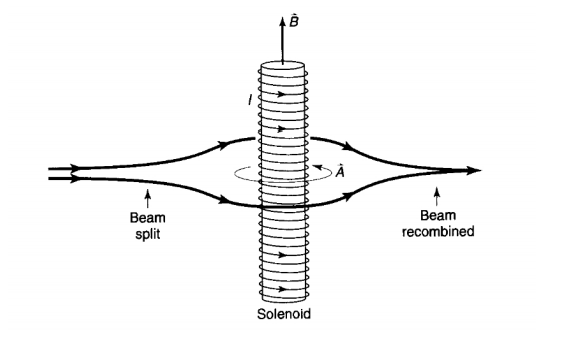
\includegraphics[scale=0.75]{bohm.png}
\end{figure}
When we turn the current on, there is a magnetic field $\mathbf{B}$ confined within the solenoid, i.e., there is no lateral magnetic field $\mathbf{B}$ on the side of the solenoid. So, according to the figure, electrons pass through a magnetic-field-free region before landing on the detector sheet. However, there exists a vector potential $\mathbf{A}$ outside of the solenoid, as the curl of $\mathbf{A}$ has to be such that the produced magnetic field $\mathbf{B}$ is contained within the coil. This can be illustrated mathematically by Stokes' theorem:
\begin{align*}
\int_D \mathbf{B}\cdots \,d\mathbf{\sigma} = \int_{\sigma D}\mathbf{A}\cdot\,d\mathbf{x}.
\end{align*}
The perturbed wavefunction as a result of passing through this region is
\begin{align*}
\psi = \psi^0_1 e^{iS_1\hbar} + \psi^0_2 e^{iS_2/\hbar}
\end{align*}
where 
\begin{align*}
S_i = e\int_{\text{path } i}\mathbf{A}\cdot\,d\mathbf{x}.
\end{align*}
It is clear now that the two components of the perturbed wavefunction has a phase difference of
\begin{align*}
\phi = \frac{S_1-S_2}{\hbar} = \frac{e}{\hbar}\oint \mathbf{A}(\mathbf{x})\cdot\, d\mathbf{x} = \frac{e}{\hbar}\oint A^\mu\,dx_\mu,
\end{align*}
which is dependent on the vector potential $\mathbf{A}$. Therefore, there is a physical effect from $\mathbf{A}$ even though the electrons do not experience any electromagnetic force. 

\subsubsection{Path-dependent Phase Factors}
Results from the Aharonov-Bohm experiment showed that knowing the electromagnetic field strength tensor $F^{\mu\nu}$ is not enough to determine all electrodynamic phenomena in quantum mechanics. In fact, a phase factor of the form
\begin{align*}
e^{\frac{-ie}{\hbar}\oint A^\mu\,dx_\mu}
\end{align*}
must be known in order to give correct predictions. Notice that the given integral is path-dependent line integral. 

\subsection{Phase Invariance in Field Theory}
Consider the Lagrangian for the free complex scalar field: 
\begin{align*}
\lag = \vert \p^\mu \phi \vert^2 = m^2\vert \psi \vert^2 
\end{align*}

\begin{align*}
(\square + m^2)\phi(x) &= 0\\
(\square + m^2)\phi^*(x) &= 0
\end{align*}

\subsection{Feynman Rules for Electromagnetism}




\newpage
\section{Lagrangian Field Theory in Flat Spacetime}
\subsection{Real Scalar Fields}
A scalar field can be used to describe particles of spin 0. A scalar field has only one component, or one degree of freedom, making it the ``simplest case'' of the fields we will discuss. Let us now consider a moving field in one dimension, which has the form
\begin{align*}
\phi(s) \sim e^{-i\mathbf{k}\cdot\mathbf{x}},
\end{align*}
where
\begin{align*}
\mathbf{k} &= K^\mu = (K^0, \vec{K})\\
\mathbf{x} &= X^\mu = (X^0, \vec{X}).
\end{align*}
Remember that $K^\mu$ is the wavenumber vector, and $X^\mu$ is the position vector. Also recall that the metric is Minkowskian at this point of consideration (we are still in flat spacetime. General curved spacetime will come later):
\begin{align*}
\eta_{\mu\nu} = \begin{pmatrix}
1 & 0 & 0 & 0\\
0 & -1 & 0 & 0\\
0 & 0 & -1 & 0\\
0 & 0 & 0 & -1
\end{pmatrix}.
\end{align*} 
Doing the inner product of $X^\mu$ and $K^\mu$ gives
\begin{align*}
\phi(x) = e^{-iK^0t + i\vec{k}\cdot\vec{x}}.
\end{align*}
We shall choose ``natural units'' such that $\hbar = c = 1$. This gives
\begin{align*}
\phi(x) = e^{-i\omega t}e^{i\vec{k}\cdot\vec{x}}.
\end{align*}
Now, particles obey the following Einstein mass-energy equivalence:
\begin{align*}
E^2 = m^2 + \vec{p}^2.
\end{align*}
But because of our choice of units, $E = c\hbar K^0= K^0$, and $\vec{p} = \hbar \vec{k} = \vec{k}$. This gives
\begin{align*}
\left( K^0\right)^2 - \vec{k}^2 &= m^2\\
K^\mu K_\mu &= m^2.
\end{align*}
So, massive particles obey $K^\mu K_\mu = m^2$, while massless particles obey $K^\mu K_\mu = 0$. \\

Now, we might wonder how we know that the scalar field has the above form. The answer is derived from, you guessed it, the Lagrangian for a scalar field. Let us consider a single scalar field in classical mechanics where
\begin{align*}
\text{Kinetic energy: } K &= \frac{1}{2}\dot{\phi}^2\\
\text{Gradient energy: } G &= \frac{1}{2}\left(\nabla \phi \right)^2\\
\text{Potential energy: } P &= V(\phi).
\end{align*}
\textit{Note: I haven't found a satisfactory explanation to what a ``gradient energy'' is. I'll come back to this term later.} \\

We currently have three terms, but we would like our Lagrangian density to have the form $\mathcal{L} = K-V$. So, let us combine the kinetic energy and gradient energy terms into one:
\begin{align*}
K' = \frac{1}{2}\dot{\phi}^2 - \frac{1}{2}\left(\nabla \phi \right)^2.
\end{align*}
We shall verify that 
\begin{align*}
K' = -\frac{1}{2}\left( \partial_\mu \phi\right)\left( \partial^\mu \phi\right) = \frac{1}{2}\dot{\phi}^2 - \frac{1}{2}\left(\nabla \phi \right)^2.
\end{align*}
This turns out to be quite straightforward:
\begin{align*}
\left( \partial_\mu \phi\right)\left( \partial^\mu \phi\right) &= \eta^{\mu\nu}\left( \partial_\mu \phi\right)\left( \partial_\nu \phi\right)\\
&= \left( \partial_0 \phi \right)^2 - \left(\partial_j\phi \right)^2\\
&= \dot{\phi}^2 - \left( \nabla \phi \right)^2.
\end{align*}
So, a good choice of Lagrangian for our scalar field would be
\begin{align*}
\mathcal{L} \sim K'-V = -\frac{1}{2}\left( \partial_\mu \phi\right)\left( \partial^\mu \phi\right) - V(\phi).
\end{align*}
In order for the action to be extremized, i.e. $\delta S = 0$, we require that $\delta \mathcal{L} = 0$ for any $\delta \phi$. Varying $\mathcal{L}$ with respect to $\phi$ gives
\begin{align*}
\delta \mathcal{L} &= \delta\left( -\frac{1}{2}\left( \partial_\mu \phi\right)\left( \partial^\mu \phi\right) - V(\phi)  \right)\\
&= -\frac{1}{2}\left( \partial_\mu \delta\phi\, \partial^\mu\phi + \partial_\mu\phi\,\partial^\mu\delta \phi \right) - \frac{dV(\phi)}{d\phi}\delta \phi\\
&= -\partial_\mu\delta \phi\, \partial^\mu\phi - \frac{dV(\phi)}{d\phi}\delta \phi.
\end{align*}
Now, integration by parts tells us that
\begin{align*}
\partial_\mu\left( \partial^\mu \phi\, \delta \phi \right) = \partial^\mu\partial_\mu\phi\, \delta \phi + \partial_\mu\delta\phi \,\partial^\mu\phi.
\end{align*}
So,
\begin{align*}
 \partial_\mu\delta \phi\, \partial^\mu\phi = \partial_\mu\left( \partial^\mu \phi\, \delta \phi \right) - \partial^\mu\partial_\mu\phi\, \delta \phi.
\end{align*}
Therefore, variations on $\mathcal{L}$ is:
\begin{align*}
\delta \mathcal{L} &= -\left[ \partial_\mu\left( \partial^\mu \phi\, \delta \phi \right) - \partial^\mu\partial_\mu\phi\, \delta \phi \right] - \frac{dV(\phi)}{d\phi}\delta \phi.
\end{align*}
It follows that the action is
\begin{align*}
S = \int_a^b \delta \mathcal{L}\,d^4x = \int^b_a \left\{ 
-\left[ \partial_\mu\left( \partial^\mu \phi\, \delta \phi \right) - \partial^\mu\partial_\mu\phi\, \delta \phi \right] - \frac{dV(\phi)}{d\phi}\delta \phi \right\}\,d^4x.
\end{align*}
The total derivative term $\partial_\mu\left( \partial^\mu \phi\, \delta \phi \right)$ vanishes as we require the variations $\delta \phi = 0$ at $a$ and $b$. This leaves us with
\begin{align*}
S = \int_a^b \left\{ 
 \partial^\mu\partial_\mu\phi - \frac{dV(\phi)}{d\phi} \right\}\,\delta \phi \,d^4x.
\end{align*}
We require that this equality hold for any variation $\delta \phi$. So it must be true that
\begin{align*}
\partial^\mu\partial_\mu\phi - \frac{dV(\phi)}{d\phi} = 0.
\end{align*}
We introduce a new operator, the \textbf{d'Alembertian}:
\begin{align*}
\square \equiv \partial^\mu\partial_\mu \equiv \partial_\nu\partial^\mu \equiv \frac{\partial^2}{\partial t^2} - \vec{\nabla}^2.
\end{align*}
The requirement we just derived now becomes the \textbf{Klein-Gordon equation}:
\begin{align*}
\square \phi - \frac{dV}{d\phi} = 0.
\end{align*}
Remember that we are working with Lagrangian for a scalar field. It can easily be shown the connection between the Klein-Gordon equations and Newton's second law of motion, by separating the temporal and spatial derivatives from the d'Alembertian and rewriting a few things:
\begin{align*}
\square \phi - \frac{dV}{d\phi} = \ddot{\phi} - \vec{\nabla}^2\phi - \frac{dV(\phi)}{d\phi} = 0.
\end{align*}
We can see the time second derivative on the field $\phi$ and the $\phi$-derivative on the potential field resemble ``acceleration'' and ``force'' in Newton's second law.\\

Let us return to our original question of why a scalar field has the form $\phi  \sim e^{-i\mathbf{k}\cdot\mathbf{x}}$. From our derivation of the Klein-Gordon equation, we observe that a scalar field $\phi$ must be a solution to the Klein-Gordon equation. Now, we verify that
\begin{align*}
\phi = e^{-i\mathbf{k}\cdot\mathbf{x}}
\end{align*}
is a solution to the KG equation. Note that even though we are concerned with real scalar field for the time being, it is reasonable to have $\phi$ of that particular complex form, simply because it makes taking derivatives easier. One can certainly work with only the real part of $\phi$ and get the same result. Now, to check when $\phi$ satisfies the Klein-Gordon equation, we simply unpack the d'Alembertian and attack the derivatives step-by-step. The first derivative is
\begin{align*}
\partial_\mu \phi &= \partial_\mu \left(e^{-i\mathbf{k}\cdot\mathbf{x}} \right)\\
&= -i\partial_\mu \left( \mathbf{k}\cdot\mathbf{x}\right)e^{-i\mathbf{k}\cdot\mathbf{x}}
\\
&= -i\partial_\mu \left(K_\nu X^\nu\right) e^{-iK_\alpha X^\alpha}\\
&= -iK_\nu\, \partial_\mu X^\nu\,\phi\\
&= -iK_\nu \delta^\nu_\mu \phi\\
&= -iK_\mu \phi 
\end{align*} 
Next, we attack the second derivative:
\begin{align*}
\partial^\mu \partial_\mu \phi &= \eta^{\mu\nu}\partial_\nu\partial_\mu\phi\\
&= \eta^{\mu\nu}\partial_\nu \left( -iK_\mu\phi \right)\\
&= -iK_\mu\eta^{\mu\nu}\left( -iK_\nu\phi \right)\\
&= (-i)^2 K^\mu K_\mu \phi.
\end{align*}
If $K^\mu K_\mu = m^2$ (as we have shown before), then 
\begin{align*}
\square \phi + m^2\phi = (-m^2 + m^2)\phi = 0, 
\end{align*}
which satisfies the Klein-Gordon equation. So, as long as $K^\mu K_\mu = m^2$ is satisfied, $\phi$ of the given form is a solution to the KG equation and is a legitimate scalar field. \\

Without knowing the solution to the Klein-Gordon equation, we can also verify that the Klein-Gordon equation is the equation of motion via the Euler-Lagrange equation, which says that
\begin{align*}
\frac{\p \lag}{\p \phi} - \p_\mu\left( \frac{\p \lag}{\p(\p_\mu \phi)} \right) = 0.
\end{align*}
Recall the Lagrangian:
\begin{align*}
\lag = \frac{1}{2}(\p_\mu\phi)(\p^\mu\phi) - V(\phi),
\end{align*}
we get
\begin{align*}
\frac{\p\lag}{\p\phi} &= -\frac{dV}{d\phi}\\
\frac{\p\lag}{\p(\p_\mu\phi)} &= \p^\mu\phi.
\end{align*}
So the Euler-Lagrange equation gives:
\begin{align*}
-\frac{dV}{d\phi} - \p_\mu(\p^\mu\phi) = 0.
\end{align*}
If we reasonably take
\begin{align*}
V(\phi) = \frac{1}{2}m^2\phi^2,
\end{align*}
then we get $-m^2\phi - \square \phi = 0$, i.e.
\begin{align*}
(\square + m^2)\phi = 0.
\end{align*}

\subsection{Overview of Noether's Theorem: A Consequence of Variational Principle}
So far, we have seen quite a lot of \textit{miraculous} coincidences, such as the fact that the Lagrangian somehow gives the Klein-Gordon equation and so on. We have also made a leap of faith from our traditional point-like description of particles $x^\mu$ to field-like descriptions $\phi$ and somehow the physics hasn't changed, i.e. we recognize that if the action is unchanged by a re-parameterization of $x^\mu$ and $\phi$, then there exist one or more conserved quantities. This is the idea of Noether's theorem. In this subsection we will get an overview of Noether's theorem and apply it to illustrate conservation rules.\\

Let us go back and redefine the Lagrangian such that it also depends on $x^\mu$ - so that we take into account the interaction of $\phi$ with the space $x^\mu$:
\begin{align*}
\lag = \lag(\phi, \p_\mu\phi,x^\mu).
\end{align*}
Next, recall our earlier definition of the variation:
\begin{align*}
\phi'(x) = \phi(x) + \delta \phi(x).
\end{align*}
This definition merely compares $\phi'$ and $\phi$ at the same location in spacetime. To get the full, total variation, we define:
\begin{align*}
\Delta \phi &= \phi'(x') - \phi(x)\\
&= [\phi'(x') - \phi(x')] + [\phi(x') - \phi(x)]\\
&\approx \delta \phi + (\p_\mu \phi)\delta x^\mu.
\end{align*}
So, the variation is now
\begin{align*}
\delta S &= \int \lag(\phi',\p_\mu\phi',x'^\mu)\,d^4x' - \int \lag(\phi,\p_\mu\phi,x^\mu)\,d^4x\\
&= \int \lag(\phi',\p_\mu\phi',x'^\mu)J\left(\frac{x'}{x} \right) \,d^4x - \int \lag(\phi,\p_\mu\phi,x^\mu)\,d^4x,
\end{align*}
where $J(x'/x)$ denotes the Jacobian - or the scaling factor:
\begin{align*}
J\left(\frac{x'}{x} \right) = \det \left(\frac{\p x'^\mu}{\p x^\lambda}\right) =   \det \left(\frac{\p (x^\mu + \delta x^\mu)}{\p x^\lambda}\right).
\end{align*}
So, the variation becomes
\begin{align*}
\delta S = \int \delta \lag + \lag \p_\mu(\delta x^\mu) \,d^4x
\end{align*}
where 
\begin{align*}
\delta \lag = \frac{\p\lag}{\p\phi}\delta \phi + \frac{\p\lag}{\p(\p_\mu\phi)}\delta(\p_\mu\phi) + \frac{\p\lag}{\p x^\mu}\delta x^\mu.
\end{align*}
Now, because $\delta(\p_\mu\phi) = \p_\mu(\delta \phi)$, the action variation becomes
\begin{align*}
\delta S &= \int \left[\frac{\p\lag}{\p\phi}\delta \phi + \frac{\p\lag}{\p(\p_\mu\phi)}\p_\mu(\delta\phi) + \frac{\p\lag}{\p x^\mu}\delta x^\mu + \lag \p_\mu (\delta x^\mu)\right]\,d^4x\\
&= \int \left[\frac{\p\lag}{\p\phi}\delta \phi + \frac{\p\lag}{\p(\p_\mu\phi)}\p_\mu(\delta\phi) + \left(\frac{\p\lag}{\p x^\mu}\delta x^\mu + \lag \p_\mu (\delta x^\mu)\right)\right]\,d^4x\\
&= \int \left[\frac{\p\lag}{\p\phi}\delta \phi + \frac{\p\lag}{\p(\p_\mu\phi)}\p_\mu(\delta\phi) + \p_\mu(\lag\delta x^\mu)\right]\,d^4x.
\end{align*}
Next, let us rewrite the second term in terms of the reverse-product rule:
\begin{align*}
\frac{\p\lag}{\p(\p_\mu\phi)}\p_\mu(\delta\phi) = 
\p_\mu\left( \frac{\p\lag}{\p(\p_\mu\phi)}\delta \phi \right)
- \p_\mu\left(\frac{\p\lag}{\p(\p_\mu\phi)} \right)\delta \phi.
\end{align*}
Assume that we are integrating over some region $R$ in spacetime, the action variation becomes
\begin{align*}
\delta S &= 
\int_R \left[\frac{\p\lag}{\p\phi}\delta \phi + 
\p_\mu\left( \frac{\p\lag}{\p(\p_\mu\phi)}\delta \phi \right)
- \p_\mu\left(\frac{\p\lag}{\p(\p_\mu\phi)} \right)\delta \phi
 + \p_\mu(\lag\delta x^\mu)\right]\,d^4x\\
 &= \int_R \left\{\delta \phi \left[\frac{\p\lag}{\p\phi} -  \p_\mu\left(\frac{\p\lag}{\p(\p_\mu\phi)} \right)\right] + \p_\mu\left[\left( \frac{\p\lag}{\p(\p_\mu\phi)}\delta \phi \right) +  (\lag\delta x^\mu) \right]\right\}\,d^4x.
\end{align*}
Gauss' theorem says that integration over a divergence (recall that $\p_\mu$ denotes divergence) of a field over a region is equal to the integration of that field over the boundary of that region, so
\begin{align*}
\delta S &=
\int_R \delta \phi \left[\frac{\p\lag}{\p\phi} -  \p_\mu\left(\frac{\p\lag}{\p(\p_\mu\phi)} \right)\right]\,d^4x + 
\int_{\p R} \left[\frac{\p\lag}{\p(\p_\mu\phi)}\delta \phi +  \lag\delta x^\mu \right]\,d\sigma_\mu.
\end{align*}  
At this point, there are two routes to take. (1) If we restrict the variation to zero at the boundaries, we will end up with the Euler-Lagrange equations, which comes from setting the integrand of the first integral to zero:
\begin{align*}
\frac{\p\lag}{\p\phi} -  \p_\mu\left(\frac{\p\lag}{\p(\p_\mu\phi)} \right) = 0.
\end{align*}
(2) The other route we can take is not requiring the variation to be zero at the boundary. Doing a small ``add and subtract'' trick to the second integrand:
\begin{align*}
\frac{\p\lag}{\p(\p_\mu\phi)}\delta \phi +  \lag\delta x^\mu 
&= \frac{\p\lag}{\p(\p_\mu\phi)}[\delta \phi +(\p_\nu\phi)\delta x^\nu ]+  \lag\delta x^\mu - \frac{\p\lag}{\p(\p_\mu\phi)}\p_\nu\phi\delta x^\nu\\
&= \frac{\p\lag}{\p(\p_\mu\phi)}[\delta \phi +(\p_\nu\phi)\delta x^\nu ] - \left[ \frac{\p\lag}{\p(\p_\mu\phi)}\p_\nu\phi
- \lag\delta^\mu_\nu\right]\delta x^\nu.
\end{align*}
Recall that the total variation is defined as
\begin{align*}
\Delta \phi \approx \delta \phi + (\p_\mu \phi)\delta x^\mu.
\end{align*}
We define the second bracketed term as the \textit{energy-momentum tensor} (we will justify this later):
\begin{align*}
\theta^\mu_\nu = \frac{\p\lag}{\p(\p_\mu\phi)}\p_\nu\phi
- \lag\delta^\mu_\nu.
\end{align*}
So, once again, the action variation becomes:
\begin{align*}
\delta S = \int_R \delta \phi \left[\frac{\p\lag}{\p\phi} -  \p_\mu\left(\frac{\p\lag}{\p(\p_\mu\phi)} \right)\right]\,d^4x + 
\int_{\p R} \left[\frac{\p\lag}{\p(\p_\mu\phi)}\Delta \phi - \theta^\mu_\nu\delta x^\nu \right]\,d\sigma_\mu.
\end{align*}
Let the infinitesimal transformations be 
\begin{align*}
\Delta \phi &= \Phi_\nu \delta \omega^\nu\\
\Delta x^\mu &= X^\mu_\nu\delta \omega^\nu \approx \delta x^\mu,
\end{align*}
where $\Phi^\mu_\nu$ is a matrix and $\Phi_\nu$ is just a row vector. By requiring that $\delta S = 0$ and requiring that the Euler-Lagrange equation hold true, we get
\begin{align*}
\int_{\p R} \left[\frac{\p\lag}{\p(\p_\mu\phi)}\Delta \phi - \theta^\mu_\nu\delta x^\nu \right]\,d\sigma_\mu &= 0\\
\int_{\p R} \left[\frac{\p\lag}{\p(\p_\mu\phi)}\Phi_\nu\delta \omega^\nu - \theta^\mu_\nu X^\nu_\mu \delta \omega^\nu \right]\,d\sigma_\mu &= 0\\
\int_{\p R} \left[\frac{\p\lag}{\p(\p_\mu\phi)}\Phi_\nu - \theta^\mu_\nu X^\nu_\mu \right]\delta \omega^\nu\,d\sigma_\mu &= 0.
\end{align*}
Let us define 
\begin{align*}
J^\mu_\nu = \frac{\p\lag}{\p(\p_\mu\phi)}\Phi_\nu - \theta^\mu_\nu X^\nu_\mu.
\end{align*}
Now, because
\begin{align*}
\int_{\p R} J^\mu_\nu \delta \omega^\nu\,d\sigma_\mu = 0
\end{align*}
must hold for any arbitrary $\delta \omega^\nu$, we require
\begin{align*}
\int_{\p R}J^\mu_\nu\,d\sigma_\mu = 0.
\end{align*}
Now, recall Gauss' theorem one more time:
\begin{align*}
\int_{\p R}J^\mu_\nu\,d\sigma_\mu = \int_R \p_\mu J^\mu_\nu\,d^4x.
\end{align*}
This means $J^\mu_\nu$ is \textit{divergence-free}, i.e. $J^\mu_\nu$ is a \textit{conserved} quantity:
\begin{align*}
\p_\mu J^\mu_\nu = 0.
\end{align*}
We can think of $J^\mu_\nu$ as \textit{current}, whose existence is invariant under the given transformations. We can also calculate another conversed quantity called the ``charge''
\begin{align*}
Q_\nu = \int_\sigma J^\mu_\nu\,d\sigma_\mu.
\end{align*}
Let's look at $\mu=0$, i.e. assuming $t$ is constant:
\begin{align*}
Q_\nu = \int_VJ^0_\nu\,d^3x.
\end{align*}
Now, revisit Gauss' theorem:
\begin{align*}
\int_V \p_0 J^0_\nu\,d^3x + \int_V \p_iJ^i_\nu\,d^3x&=0\\
\int_V \p_0 J^0_\nu\,d^3x + 0 &= 0\\
\frac{d}{dt}\int_V J^0_\nu\,d^3x &= \frac{dQ_\nu}{dt} = 0.
\end{align*}
So \textit{charge} is conserved over time. This is the essence of \textit{Noether's theorem}.\\

Finally, let us justify the definition of $\theta^\mu_\nu$ as the energy-momentum tensor. We require that the laws of physics remain the same translationally, and the same in all time. So, let see what we get if we make the transformations
\begin{align*}
X^\mu_\nu &= \delta^\mu_\nu\\
\Phi_\mu &= 0.
\end{align*}
Now recall the definition of $J^\mu_\nu$, then apply the transformations to the definition:
\begin{align*}
J^\mu_\nu = \frac{\p\lag}{\p(\p_\mu\phi)}\Phi_\nu - \theta^\mu_\nu X^\nu_\mu = -\theta^\mu_\nu \delta ^\nu_\mu = -\theta^\mu_\nu.
\end{align*}
And so the conservation law, by taking $\mu=0$, is
\begin{align*}
\frac{d}{dt}\int \theta^0_\nu\,d^3x = \frac{d}{dt}P_\nu= 0.
\end{align*}
Let us calculate the first component $P_0$ from the definition of $\theta^\mu_\nu$, to show (partly) that $P_\nu$ is the 4-momentum:
\begin{align*}
P_0 = \int\theta^0_0\,d^3x = \int\left\{\frac{\p \lag}{\p(\p_0\phi)} - \lag \right\} \,d^3x = \int \left\{
\frac{\p\lag}{\p\dot{\phi}}\dot{\phi} - \lag \right\}\,d^3x. 
\end{align*}
The right-hand side the energy of the field. Next, we can show
\begin{align*}
\int \theta^0_i\,d^3x
\end{align*}
is the momentum from the fact that $\p\phi/\phi x^\mu$ is a 4-vector under Lorentz transformations. \\

Now, if we had assumed that the Lagrangian hadn't involved $x^\mu$, then we would have ended at the Euler-Lagrange equation, i.e. the system does not exchange energy and momentum with the outside. We condense that with the following proposition:\\

\begin{prop}
	Conservation of energy and momentum holds for a system whose Lagrangian does not depend of $x^\mu$.
\end{prop}

Now, let us look at the relationship between the energy-momentum tensor $\theta^\mu_\nu$ and the $x^\mu$-independent Lagrangian, which can be given by
\begin{align*}
\lag = \frac{1}{2}g^{\mu\nu}(\p_\mu\phi)(\p_\nu\phi) - \frac{m^2}{2}\phi^2.
\end{align*}
So $\theta^{\mu\nu}$ can be written as (some of the derivations can be found in the previous subsection):
\begin{align*}
\theta^{\mu\nu} &= g^{\lambda\nu}\theta^\mu_\lambda \\
&= g^{\lambda\nu}\left( \frac{\p\lag}{\p(\p_\mu\phi)}\p_\lambda\phi - \delta^\mu_\lambda\lag \right)\\
&= g^{\lambda\nu}(g^{\mu\lambda}(\p_\lambda\phi) - \delta^\mu_\lambda\lag)\\
&= g^{\lambda\nu}(\p^\mu\phi\,\p_\lambda\phi - \delta^\mu_\lambda\lag)\\
&= (\p^\nu\phi)(\p^\mu\phi) - g^{\mu\nu}\lag.
\end{align*}
We observe that $\mu$ and $\nu$ are exchangeable, hence $\theta^{\mu\nu}$ is symmetric. So, for a scalar field $\phi$ whose Lagrangian does not exchange energy and momentum with the external, then the energy-momentum tensor $\theta^{\mu\nu}$ is \textbf{symmetric}. However, in general $\theta^{\mu\nu}$ is not symmetric, in general, by definition. But, we can define the \textit{canonical energy-momentum tensor} as
\begin{align*}
T^{\mu\nu} = \theta^{\mu\nu} + \p_\lambda f^{\lambda\mu\nu}
\end{align*}
such that $\p_\mu T^{\mu\nu} = 0$ and $T^{\mu\nu}$ is symmetric. We will not go into detail about this, but the idea is similar to the three-dimensional case in vector calculus where the curl of a vector field is the same as the curl of that same vector field added to a gradient of some other scalar field. By adding the $f$ term, what we wish to accomplish is have $T$ be both divergence-free and symmetric. Now, why do we want the energy-momentum tensor to be symmetric? One of the reasons for this is that in general relativity, Einstein's field equation requires that the energy-momentum stress tensor be symmetric, because the Ricci tensor $R_{\mu\nu}$ and the metric tensor $g_{\mu\nu}$ are both symmetric.

\subsection{Complex Scalar Fields and Electromagnetism}
\subsubsection{Gauge transformation of the first kind - Global Symmetry}
In this section, we will see how things ``come together.'' As real scalar fields describe massive neutral particles and how vector fields describe massless photons, complex scalar fields somehow fills in and completes the picture by bringing in the charge and somehow joins the real scalar and vector field pictures. At the end of this section, we will see how the ``full theory'' where the electromagnetic field with charge is described by a single Lagrangian. \\

If our scalar field is complex, we can think of it and its complex conjugate as:
\begin{align*}
\phi &= \frac{\phi_r + i\phi_i}{\sqrt{2}}\\
\phi^* &= \frac{\phi_r - i\phi_i}{\sqrt{2}}.
\end{align*}
Or, we can think of $\phi$ and $\phi^*$ as independent fields. Since the Lagrangian has to be real, plugging $\phi$ and $\phi^*$ into the Lagrangian introduced in the previous section gives:
\begin{align*}
\lag = (\p_\mu \phi)(\p^\mu \phi)^* - m^2\phi^*\phi.
\end{align*}
Without much inspection, we can see that the fields satisfy the Klein-Gordon equation:
\begin{align*}
\begin{cases}
(\square + m^2)\phi &= 0\\
(\square + m^2)\phi^* &= 0.
\end{cases}
\end{align*}
Now, we can ask ourselves: ``Is this Lagrangian invariant under the transformation
\begin{align*}
\phi &\to e^{-i\Lambda}\phi\\
\phi^* &\to e^{i\Lambda}\phi^*,
\end{align*}
where $\Lambda$ is a constant?'' Again, by inspection, the answer is yes, simply because the transformation is nothing but an orthogonal rotation (length preserving). And since because we changed the field the same way everywhere by a rotation induced by $e^{\pm i\Lambda}$ while the Lagrangian remains invariant, we say that the theory has a \textbf{global U(1) symmetry}. Global transformations like this one are called \textit{gauge transformation of the first kind}.
\subsubsection{Gauge transformation of the second kind - Local Symmetry}
Now, consider the case where the rotation operation $e^{\pm i \Lambda}$ has a spatio-dependence, i.e., $\Lambda \to \Lambda(x)$. We call this a \textit{gauge transformation of the second kind}. This leads to the fact that $\phi$ transform differently at different places. We want our theory to also be invariant under this ``local'' transformation. But first, we have to show that our previous Lagrangian no longer retains its gauge symmetry and try to come up with ways to ``fix'' the theory. Let us say that $\phi$ transforms as $\phi \to \phi e^{i\Lambda(x)}$, then
\begin{align*}
\p_\mu \phi \to \p_\mu (\phi e^{i\Lambda(x)}) = i(\p_\mu \Lambda(x))\phi + e^{i\alpha}\p_\mu \phi.
\end{align*}
It is already clear that 
\begin{align*}
(\p_\mu \phi)(\p_\mu \phi)^* \not\to (\p_\mu \phi)(\p_\mu \phi)^* e^{i\Lambda(x)}
\end{align*}
since there will always be some $\Lambda(x)$-dependent residual terms. We can stop here and surrender, but we can also ``fix'' our notion of the derivative (just like what we did in general relativity), introducing the \textbf{gauge-covariant derivative}:
\begin{align*}
D_\mu = \p_\mu + iqA_\mu,
\end{align*}
where $q$ is the charge, which acts as a \textit{coupling term} like the Christoffel symbols in general relativity, and $A_\mu$ is the vector potential, which is also the gauge field that has symmetry:
\begin{align*}
A_\mu \sim A_\mu + \p_\mu\Lambda.
\end{align*}
Once again, recall we have discussed in the gauge invariance section. By adding the 4-dimensional gradient of a scalar field $\Lambda$ (so adding the $\p_\mu \Lambda$ term), we are not changing the 4-dimensional curl of $A_\mu$, i.e. the electromagnetic field tensor $F^{\mu\nu}$ is divergence-free. We can refer to section on gauge invariance for more details about this is true. But focusing on the results here, if we cleverly (once again) pick $\Lambda$ such that
\begin{align*}
\Lambda(x) = -\frac{\alpha(x)}{q}
\end{align*}
then with the gauge transformations
\begin{align*}
\begin{cases}
\phi \to \phi e^{i\Lambda(x)}\\
A_\mu \to A_\mu - \frac{1}{q}\p_\mu\Lambda(x)
\end{cases}
\end{align*}
the new derivative $D_\mu\phi = (\p_\mu + iqA_\mu)\phi$ is transformed into
\begin{align*}
&\to \left( \p_\mu  iq\left[ A_\mu -\frac{1}{q}\p_\mu\Lambda(x)  \right] \right)\phi e^{i\Lambda(x)}\\
&= e^{i\Lambda(x)}\left( \p_\mu\phi + i(\p_\mu\Lambda(x)\phi) + iqA_\mu \phi - i(\p_\mu \Lambda(x))\phi \right)\\
&= e^{i\Lambda(x)}(\p_\mu \phi + iqA_\mu\phi)\\
&= e^{i\Lambda(x)}D_\mu\phi.
\end{align*}
So, $D_\mu\phi$ transforms correctly. Since we have added the electromagnetic vector potential to the theory, adding the electromagnetic field tensor term completes the classical field theory for the charged scalar field in electromagnetism. 
\begin{align*}
\boxed{\lag = \vert D_\mu \phi\vert^2 - m^2\vert \phi\vert^2 - \frac{1}{4}F_{\mu\nu}F^{\mu\nu} }
\end{align*}


\subsection{Vector Fields and Photons}

In this section, we will see how electromagnetism naturally arises from the previous section where we demand invariance of the action under gauge transformation of the second kind (local rotations). In particular, we will work with a Lagrangian density that describes the massless and neutral photon, and see how variations on the action gives rise to the Maxwell's equations. We will also confirm that fact that photons must be massless in the theory, by enforcing conditions on the vector potential $A_\mu$. The section is more of synopsis of the methods we have learned so far about variations on the action, gauge transformations, symmetries, and invariances. The goal of this section is to show the theory actually works to describe a physical, real, particle. We will be working with vector field in the formulation the action, but the main principles regarding variations and gauge-stuff are the same.  \\

Vector fields describe particles of spin 1 such as photons. Unlike real scalar fields $\phi$ where there is only one degree of freedom, a vector field is represented by $A_\mu$ with $\mu = 0,1,2,3$, hence having 4 degrees of freedom. Electromagnetism is a field theory where the relevant field is a vector field, $A_\mu$, called the vector potential.
\begin{align*}
A_\mu = (A_0, \vec{A}).
\end{align*}
The first component of the vector potential, $A_0$ is the electrostatic potential $V$ where $\vec{E} = -\vec{\nabla}V$. The other spatial components of $A_\mu$, forming $\vec{A}$, form the vector potential from which the magnetic field and full electric field is derived:
\begin{align*}
\vec{B} &= \vec{\nabla}\times \vec{A}\\
\vec{E} &= -\vec{\nabla}V - \frac{\partial \vec{A}}{\partial t}
\end{align*}

Let us consider the following Lagrangian density:
\begin{align*}
\mathcal{L} = -\frac{1}{4}F_{\mu\nu}F^{\mu\nu} - j^\mu A_\mu,
\end{align*}
where $j^\mu = (\rho, \vec{J})$ is a combination of the charge density and current density. The electromagnetic field strength tensor is given by:
\begin{align*}
F^{\mu\nu} &= \partial^\mu A^\nu - \partial^\nu A^\mu \\
&= \begin{pmatrix}
0 & -E^1 & -E^2 & -E^3\\
E^1 & 0 & -B^3 & B^2 \\
E^2 & B^3 & 0 & -B^1\\
E^3 & -B^2 & B^1 & 0
\end{pmatrix}.
\end{align*}
With this definition, we can also have an equivalent definition:
\begin{align*}
F_{\mu\nu} = \partial_\mu A_\nu - \partial_\nu A_\mu.
\end{align*}
Recall the cyclic identity (this can be readily verified - we in fact have covered this in the GR notes):
\begin{align*}
\partial_\lambda F_{\mu\nu} + \partial_{\mu}F_{\nu\lambda} + \partial_{\nu}F_{\lambda\mu} = 0.
\end{align*}
We can easily show that this identity yields two of four Maxwell's equations:
\begin{align*}
\vec{\nabla}\times\vec{E} &= -\frac{\partial \vec{B}}{\partial t}\\
\vec{\nabla}\cdot\vec{B} &= 0.
\end{align*}
The remaining Maxwell equations come from varying the action and minimizing the action: $\delta S = 0$ with respect to the vector potential $A_\mu$. Similar to what we have done before, we want to vary the Lagrangian. Now, the E\&M Lagrangian has two terms. The term involving the vector potential is simple:
\begin{align*}
\delta \left( j^\mu A_\mu \right) = j^\mu\,\delta A_\mu 
\end{align*}
true for all $\delta A_\mu$, so if the field strength tensor is zero, then $j^\mu = 0$. The term involving the field strength tensor is a little more complicated, but certainly doable:
\begin{align*}
\delta\left( \frac{-1}{4}F^{\mu\nu}F_{\mu\nu} \right) 
&= \frac{-1}{4}\,\delta\left[\left( \partial^\mu A^\nu - \partial^\nu A^\nu  \right)\left( \partial_\mu A_\nu - \partial_\nu A_\mu \right)\right]\\
&= \frac{-1}{2}\,\delta\left( \partial^\mu A^\nu\,\partial_\mu A_\nu - \partial_\mu A_\nu\,\partial^\mu A^\nu\right)\\
&= \frac{-1}{2}\left( \partial^\mu\,\delta A^\nu\,\partial_\mu A_\nu  + 
\partial^\mu A^\nu\,\partial_\mu\,\delta A_\nu - \partial_\mu \,\delta A_\nu\,\partial^\mu A^\nu - \partial_\mu  A_\nu\,\partial^\mu \,\delta A^\nu \right).
\end{align*}
Raising and lowering indices gives
\begin{align*}
\delta\left( \frac{-1}{4}F^{\mu\nu}F_{\mu\nu} \right)  
&= \frac{-1}{2}\left( 
\partial^\mu\,\delta A^\nu\,\partial_\mu A_\nu  + 
\partial_\nu A_\mu\,\partial^\nu\,\delta A^\mu 
- \partial_\mu \,\delta A_\nu\,\partial^\mu A^\nu 
- \partial^\nu A^\mu\,\partial_\nu \,\delta A_\mu \right)\\
&= \partial^\nu\,\delta A^\mu\,\partial_\nu A_\mu - \partial_\mu \,\delta A_\nu\,\partial^\mu A^\nu.
\end{align*}
We can again integrate by parts on the two terms similar to the following steps
\begin{align*}
\partial^\nu\,\delta A^\mu\,\partial_\nu A_\mu &=  \partial^\nu(\partial_\mu A_\nu\,\delta A^\mu) -(\partial^\nu\partial_\mu A_\nu)\delta A^\mu = \partial_\mu(\partial^\nu A^\mu\,\delta A_\nu) -(\partial^\nu\partial_\mu A_\nu)\delta A^\mu
\\
\partial_\mu\,\delta A_\nu\partial^\mu A^\nu &= 
\partial_\mu (\partial^\mu A^\nu \,\delta A_\nu)
 - \partial_\mu(\partial^\mu A^\nu)\,\delta A_\nu  =
\partial_\mu (\partial^\mu A^\nu \,\delta A_\nu) 
 - \partial_\mu(\partial^\mu A^\nu)\,\delta A_\nu.
\end{align*} 
and eliminate the total derivative from the action integral. Assuming that the term with the current density and vector potential is zero, we are eventually (after lowering/raising the indices correctly, of course) left with the requirement
\begin{align*}
\partial_\mu(\partial^\mu A^\nu)\,\delta A_\nu - (\partial^\nu\partial_\mu A_\nu)\delta A^\mu
&\equiv 
\left(\square A^\mu - \partial^\mu\partial^\nu A_\nu \right)\,\delta A_\mu = 0
\end{align*}
for all $\delta A_\mu$, which forces the following identity:
\begin{align*}
\square A^\mu - \partial^\nu \partial^\mu A_\nu = \square A^\mu - \partial_\nu \partial^\mu A^\nu = \partial_\nu(\partial^\nu A^\mu - \partial^\mu A^\nu) = \partial_\nu F^{\mu\nu} = 0.
\end{align*}
Now, with the current density and vector potential terms, we get the requirement 
\begin{align*}
\partial_\nu F^{\mu\nu} = j^\mu. 
\end{align*}
This identity gives the remaining two Maxwell's equations.\\

We can look at photons as an example. Photons do not carry a current/charge, so $j^\mu = 0$. Therefore the equation of motion can be derived from just
\begin{align*}
\partial_\nu F^{\mu\nu} = 0.
\end{align*}
Now, we have an interesting problem to think about: We know that photons can have 2 independent transverse polarizations, i.e. there are 2 massless modes for photons. However, $A^\mu$ has 4 degrees of freedom, not 2. So why does our theory require more than 2 degrees of freedom to describe a physical quantity that only has 2 degrees of freedom? The answer to this is that there are 2 degrees of freedom in $A_\mu$ that don't matter. The first is the $A_0$ factor - the electrostatic potential. Why $A_0$ does not matter in describing photons can be illustrated if we look at the case where $\mu = 0$:
\begin{align*}
\square A_0 - \partial_0\,\partial^\nu A_\nu 
&= \partial^0\partial_0A_0 + \partial^j\partial_jA_0 - \partial_0\partial^0A_0-\partial_0\partial^jA_j\\ 
&=  \partial^j\partial_jA_0 - \partial_0\partial^jA_j \\
&=  0.
\end{align*} 
We see that $A_0$ is not a propagating mode, or the \textbf{ghost} mode, or the \textbf{auxiliary} mode. This is actually a good thing in our theory. In fact, the Lagrangian is actually chosen such that the time second derivative vanishes. \\

Now that we have sort of explained why one degree of freedom of $A_\mu$ does not matter. What about the other one that shouldn't matter? The short answer to this is the keyword \textbf{gauge symmetry} in the theory. If we look back at how the field strength tensor is defined as the 4-dimensional curl of the vector potential $A_\mu$:
\begin{align*}
F_{\mu\nu} = \partial_\mu A_\nu - \partial_\nu A_\mu.
\end{align*}
As an aside, it makes sense to define the 4-dimensional curl this way, because the curl of a 2-vector field in two dimensions gives a scalar (a zero-index object), the curl of a 3-vector field in three dimensions gives a 3-vector field (a one-index object). So it is reasonable to define the 4-dimensional curl of a 4-vector field as a tensor (a two-index object). Now, back to our problem. We should also attempt to gauge transform
\begin{align*}
A_\mu \rightarrow A'_\mu = A_\mu + \partial_\mu\Lambda(x),
\end{align*}
then we observe that
\begin{align*}
F'_{\mu\nu} &= \partial_\mu(A_\nu + \partial_\nu\Lambda(x)) - \partial_\nu(A_\mu + \partial_\mu\Lambda(x))\\
 &= \partial_\mu A_\nu - \partial_\nu A_\mu \\
 &= F^{\mu\nu},
\end{align*}
i.e. there is a way to choose $\Lambda(x)$ such that we eliminate one $A_\mu$ mode, leaving just 4-1-1=2 modes.\\

The goal of the above gauge transformation is to pick a $\Lambda(x)$ to remove an extra degree of freedom in the theory. Let us suppose that $\p^\mu A_\mu \neq 0$, i.e. $A_\mu$ is NOT divergence-free. We can pick $\Lambda(x)$ such that after the transformation, $\p^\mu A'_\mu = 0$. Let's start from the very beginning, repeat what we just done earlier:
\begin{align*}
A'_\nu = A_\nu + \p_\nu\Lambda.
\end{align*}
It follows that
\begin{align*}
\p^\nu A'_\nu &= \p^\nu(A_\nu + \p_\nu\Lambda)\\
&= \p^\nu A_\nu + \p^\nu \p_\nu \Lambda\\
&= \p^\nu A_\nu + \square\Lambda.
\end{align*}
This suggests that if we pick $\Lambda(x)$ such that $\square\Lambda(x) = -\p^\nu A_\nu$ then in this gauge $\p^nu A'_\nu = 0$. After that, we can just drop the prime and get $\p^\nu A_\nu = 0$. As a consequence, in this fixed gauge, the equations of motion can be deduced from 
\begin{align*}
\begin{cases}
\square A_\mu = 0\\
\p^\nu A_\nu = 0
\end{cases}
\end{align*}
each of which adds one constraint, reducing the degree of freedom by 1. To solve for $A_\mu$, we can assume the form of $A_\mu$:
\begin{align*}
A_\mu = \epsilon_\mu e^{-i\mathbf{k}\cdot\mathbf{x}},
\end{align*}
where $\epsilon_\mu$ is called the \textbf{polarization vector}. Now, let us work with the first constraint $\square A = 0$. We can verify (below) that this constraint requires $K^\mu K_\mu = 0$, i.e. $K^\mu$ is a null vector in flat Minkowskian spacetime, i.e. it is light-like. 
\begin{align*}
\square A_\mu &= \p_\mu \p^\mu A_\mu\\
&= \p_\mu\left( 
\eta^{\mu\nu}\p_\nu \epsilon_\mu e^{-i\mathbf{k}\cdot\mathbf{x}}
\right)\\
&= \p_\mu\left[\epsilon_\mu\eta^{\mu\nu}\left(\p_\nu  e^{-i\mathbf{k}\cdot\mathbf{x}}
\right)\right]\\
&= \p_\mu\left[\epsilon_\mu\eta^{\mu\nu}(-iK_\mu)\left(
e^{-i\mathbf{k}\cdot\mathbf{x}}\p_\nu X^\mu
\right)\right]\\
&= \p_\mu\left[\epsilon_\mu\eta^{\mu\nu}(-iK_\mu)\left(
e^{-i\mathbf{k}\cdot\mathbf{x}}\delta^\mu_\nu
\right)\right]\\
&= (-iK^\nu)\p_\mu A_\mu\\
&= 4(-iK^\nu)(-iK_\mu)A_\mu\\
&= 4(-i)^2 K_\mu K^\mu A_\mu\\
&= 0 \text{ if } K_\mu K^\mu = 0.
\end{align*}
This requirement implies that the vector field $A_\mu$ is massless ($K^\mu K_\mu = 0$ rather than $m^2$ like in the scalar field example), which is a good thing, since we are working with electromagnetism and these mathematical objects ultimately describe electromagnetic waves - photons. \\

Next, the other constraint $\p^\nu A_\nu = 0$ motivates us to choose $\Lambda$ such that
\begin{align*}
\square \Lambda = -\p^\nu A_\nu
\end{align*}
so that $\p^\nu A'_\nu = 0$. However, this isn't enough information to choose $\Lambda$, because $\square \Lambda = -\p^\nu A_\nu$ alone cannot fix $\Lambda$. We also have to look at the gauge transformation of $A_\mu$ and make sure that the auxiliary part $A_0$ vanishes, then we have enough information to pick $\Lambda$. Let us start with the form of $A_\mu$:
\begin{align*}
A_\mu = \epsilon_\mu e^{-i\mathbf{k}\cdot\mathbf{x}}.
\end{align*}
We know that $\square A_\mu = 0$, so if we pick
\begin{align*}
\Lambda = \lambda e^{-i\mathbf{k}\cdot\mathbf{x}}
\end{align*}
then we are guaranteed $\square \Lambda = 0 = \p^\nu A_\nu$. So that is quite nice. But what is $\lambda$? We can only set $\lambda$ if we fix the value of $A_0$. It makes sense to set $A_0 = 0$ so that it vanishes. With this, we can perform a gauge transformation on $A_0$, set it to zero, and find $\lambda$:
\begin{align*}
A_0 &\rightarrow A_0 + \p_0 \Lambda = 0\\
&\rightarrow e^{-i\mathbf{k}\cdot\mathbf{x}}(\epsilon_0 - i\lambda K_0) = 0\\
&\rightarrow \lambda = \frac{\epsilon_0}{i K_0}. 
\end{align*}
So, if we pick 
\begin{align*}
\Lambda = \frac{\epsilon}{i K_0}e^{-i\mathbf{k}\cdot\mathbf{x}}
\end{align*}
then $A_0 = 0$ implies
\begin{align*}
\p^\nu A_\nu = \p^0 A_0 + \vec{\nabla}\cdot\vec{A} = \vec{\nabla}\cdot\vec{A} = 0.
\end{align*}
So, it turns out that we can simply complete gauge fixing by setting two additional constraints on $A_\mu$:
\begin{align*}
\begin{cases}
A_0 = 0\\
\vec{\nabla}\cdot\vec{A} = 0,
\end{cases}
\end{align*}
i.e., we require that the vector potential $A_\mu$ be divergence-free and to have a vanishing auxiliary mode. With this, we can the degree of freedom of $A_\mu$ from 4 from 2, making it a physical description. We shall show that can be done now. If we revisit the polarization vector
\begin{align*}
\epsilon_\mu = (\epsilon_0, \epsilon_1, \epsilon_2, \epsilon_3)
\end{align*}
and require that $A_0 = 0$, then obviously $\epsilon_0 = 0$. But since we also require $\vec{\nabla}\cdot\vec{A} = 0$, we have
\begin{align*}
\vec{\nabla}\cdot\vec{A} &= \p_j A^j\\
&= \p_j \left( \epsilon^j e^{-i\mathbf{k}\cdot\mathbf{x}} \right)\\
&\propto A^j (-iK_j)\\
&= 0.
\end{align*}
So, $\vec{k}\cdot\vec{A} = 0$, i.e., they are orthogonal vectors. Now, consider a photon traveling in the $z$-direction. Because $K_\mu k^\mu = 0$, we have
\begin{align*}
K^\mu = (K,0,0,K).
\end{align*}
Because $\vec{k}\cdot\vec{A} \propto \vec{k}\cdot\vec{\epsilon}$, it follows that $K\epsilon^3 = 0$, i.e., there is no longitudinal component in the polarization vector. Therefore,
\begin{align*}
\epsilon_\mu = (0, \epsilon_1, \epsilon_2, 0).
\end{align*}
So, the vector potential $A_\mu$ has the form
\begin{align*}
A_\mu = \epsilon_\mu e^{-i\mathbf{k}\cdot\mathbf{x}} = \begin{pmatrix}
0\\\epsilon_1\\\epsilon_2\\0
\end{pmatrix}e^{-i\mathbf{k}\cdot\mathbf{x}}.
\end{align*}
We can construct the independent modes of propagation as
\begin{align*}
\begin{cases}
\epsilon^{(1)}_\mu = (0,1,0,0)^\top\\
\epsilon^{(2)}_\mu = (0,0,1,0)^\top,
\end{cases}
\end{align*}
which give two physical transverse modes of the vector potential
\begin{align*}
\begin{cases}
A^{(1)}_\mu = (0,1,0,0)^\top e^{-i\mathbf{k}\cdot\mathbf{x}} = \epsilon^{(1)}_\mu e^{-i\mathbf{k}\cdot\mathbf{x}}\\
A^{(2)}_\mu = (0,0,1,0)^\top e^{-i\mathbf{k}\cdot\mathbf{x}} = 
\epsilon^{(2)}_\mu e^{-i\mathbf{k}\cdot\mathbf{x}},
\end{cases}
\end{align*}

All is good, but we might wonder why photons are massless. The answer depends on who we ask, but mathematically, it is the gauge symmetry requirement that ``makes'' photons massless. Suppose that the Lagrangian is of the form
\begin{align*}
\lag = -\frac{1}{4}F_{\mu\nu}F^{\mu\nu}+ \frac{1}{2}m^2A_\mu A^\mu,
\end{align*}
which suggests that the field is massive (hence the mass term $m$). Under gauge transformation,
\begin{align*}
A_\mu \rightarrow A_\mu + \p_\mu \Lambda,
\end{align*}
we have 
\begin{align*}
\begin{cases}
F_{\mu\nu} \rightarrow F_{\mu\nu}\\
A_\mu A^\mu = (A_\mu + \p_\mu\Lambda)(A^\mu + \p^\mu\Lambda) \not\to A_\mu A^\mu
\end{cases}
\end{align*}
So, the Lagrangian is no longer gauge-invariant. Therefore we claim that massive fields do not have gauge symmetry, i.e., we cannot have the mass term if we require mass invariance:
\begin{align*}
\text{Massless field }\iff \text{ Gauge invariance}.
\end{align*}
This also hints to us that mass comes from some mechanism that breaks gauge symmetry, which we will explore later on. 

\newpage

\section{Symmetries and Conservation Laws}

\newpage

\section{Gravitation and Lagrangian Formulation of General Relativity}

\subsection{Review of General Relativity \& Curved Spacetime}

\subsubsection{General Relativity}
Taking the speed of light, $c$, to be 1, the Einstein equation for general relativity is
\begin{align*}
R_{\mu\nu} - \frac{1}{2}Rg_{\mu\nu} = 8\pi GT_{\mu\nu}.
\end{align*}
Sometimes, it is more useful to write the Einstein's equation as
\begin{align*}
R_{\mu\nu} = 8\pi G \left( T_{\mu\nu} - \frac{1}{2}Tg_{\mu\nu} \right).
\end{align*}
In vacuum, where all components of the energy-momentum stress tensor are zero, the Einstein's equation becomes
\begin{align*}
R_{\mu\nu} = 0.
\end{align*}

\subsubsection{Curved Spacetime}
Perhaps the most important change as we go from flat to general curved spacetime is the notion of the ``derivative.'' In introduction to general relativity, we have introduced the \textbf{covariant derivative} and \textbf{absolute derivative}. We shall revisit the covariant derivative, as it will be important in the derivation of Lagrangian formulation of gravitation. The covariant derivative has the form - or forms, should I say:
\begin{align*}
D_\mu w_\nu &= \p_\mu w_\nu - \Gamma^\lambda_{\mu\nu}w_\lambda\\
D_\mu v^\nu &= \p_\mu v^\nu + \Gamma^\nu_{\lambda\nu}v^\lambda.
\end{align*}
Note the sign difference in the definitions. The covariant derivative is defined \textit{differently} for covariant and contravariant vectors. In fact, this follows if we define the covariant derivative for one kind of vectors.
\begin{propty}
	Strictly speaking, some of theses properties are required for the definition of the covariant derivative to make sense and work. 
	\begin{enumerate}
		\item Linearity: $D(U+V) = D(U) + D(V)$
		\item Product rule: $D(U\otimes V) = D(U)\otimes D(V)$
		\item Commutes with contractions: $D_\mu(\tensor{T}{^{\lambda}_{\lambda\rho}}) = \tensor{(DT)}{_\mu^\lambda_{\lambda\rho}}$
	\end{enumerate}
\end{propty} 
Next, recall the definition of the \textbf{Christoffel symbol}:
\begin{align*}
\Gamma^{\lambda}_{\mu\nu} = \frac{1}{2}g^{\lambda\rho}\left(
   \p_{\mu}g_{\rho\nu}
 + \p_{\nu}g_{\mu\rho}
 - \p_{\rho}g_{\mu\nu}
 \right).
\end{align*}
Now, consider a contravariant vector $V^\mu$, we can define the \textbf{divergence} in curved spacetime based on the flat 3-space definition
\begin{align*}
\text{div}\vec{V} = \p_i V^i
\end{align*}
by ``contracting'' an index and adding the Christoffel symbols:
\begin{align*}
D_\mu V^\mu = \p_\mu V^\mu + \Gamma^\mu_{\mu\lambda}V^\lambda.
\end{align*}
Next, invoking the definition of the Christoffel symbols, we can compute 
\begin{align*}
\Gamma^\mu_{\mu\lambda} &= \frac{1}{2}g^{\mu\rho}(\p_\mu g_{\rho\lambda} + \p_\lambda g_{\rho\mu} - \p_\rho g_{\mu\lambda})\\
&= a
\end{align*}

\subsection{Lagrangian Formulation}
The action is
\begin{align*}
S = \int \lag (\Phi^i, \nabla_\mu \Phi^i)\,d^nx.
\end{align*}
$\lag$ is a density. 
\begin{align*}
\lag = \sqrt{-g}\hat{\lag}
\end{align*}
where $\hat{\lag}$ is a scalar. The associated Euler-Lagrange equation is
\begin{align*}
\frac{\p \hat{\lag}}{\p \Phi} - \nabla_\mu \left( \frac{\p \hat{\lag}}{\p (\nabla_\mu \Phi)}\right) = 0.
\end{align*}
Recall Stokes' theorem:
\begin{align*}
\int_\Sigma \nabla_\mu V^\mu \sqrt{\vert g\vert}\,d^nx = \int_{\p\Sigma} n_\mu V^\mu \sqrt{\vert \gamma \vert},d^{n-1}x
\end{align*}

\newpage

\section{Quantization}

\newpage

\section{Worked Problems}
Consider the following Lagrangian
\begin{align*}
\lag = -\frac{1}{4}F_{\mu\nu}F^{\mu\nu} + \frac{1}{2}m^2 A_\mu A^\mu
\end{align*}
which describes a massive particle with a vector field.\\
\begin{prob}
	Verify that this Lagrangian does not have gauge symmetry under the gauge transformation $A_\mu \to A_\mu +\p_\mu \Lambda$, i.e. $\lag \not\to \lag$.\\
	\begin{sln}
		We simply brute force through the problem and show that $\lag' \neq \lag$, where:
		\begin{align*}
		\lag' = -\frac{1}{4}F_{\mu\nu}F^{\mu\nu} + \frac{1}{2}m^2 A'_\mu A'^\mu.
		\end{align*}
		Note that even though $F^{\mu\nu}$ is defined in terms of $A_\mu$, $F_{\mu\nu}$ is invariant under the gauge transformation because it is the 4-dimensional curl of $A_\mu$. We can verify this fact later. Focusing only on the massive term in the new Lagrangian:
		\begin{align*}
		\lag' &= -\frac{1}{4}F_{\mu\nu}F^{\mu\nu} + \frac{1}{2}m^2 A'_\mu A'^\mu\\
		&= -\frac{1}{4}F_{\mu\nu}F^{\mu\nu} +\frac{1}{2}m^2(A_\mu + \p_\mu \Lambda)(A^\mu + \p^\mu \Lambda)\\
		&= \lag + \frac{1}{2}m^2(A_\mu \p^\mu\Lambda + A^\mu \p_\mu \Lambda + \p_\mu\Lambda \p^\mu \Lambda)
		\end{align*}
		It is clear that our choice of the scalar field $\Lambda$ affects the form of the new Lagrangian. So, $\lag \neq \lag'$ in general. Therefore, the massive vector Lagrangian does not have gauge symmetry under the given gauge transformation.\\
		
		As an aside, we can verify that $F_{\mu\nu}\to F_{\mu\nu}$. The $F^{\mu\nu} \to F^{\mu\nu}$ identity will follow accordingly. 
		\begin{align*}
		F'_{\mu\nu} &= \p_\mu A'_\nu - \p_\nu A'_\mu\\
		&= \p_\mu(A_\nu + \p_\nu\Lambda) - \p_\nu(A_\mu + \p_\mu\Lambda)\\
		&= F_{\mu\nu} + \p_\mu \p_\nu \Lambda - \p_\nu \p_\mu\Lambda\\
		&= F_{\mu\nu},
		\end{align*}
		where $\p_\mu \p_\nu \Lambda - \p_\nu \p_\mu\Lambda=0$ because $\Lambda$ is a scalar (this is also true by index-swapping). So the electromagnetic field tensor has gauge symmetry under the given gauge transformation. \\
	\end{sln}
\end{prob}

\begin{prob}
	Vary the action
	\begin{align*}
	S = \int \lag\,d^4x
	\end{align*}
	with respect to $A_\mu$ and show that the equations of motion are 
	\begin{align*}
	\square A - \p_\mu \p^\nu A_\nu + m^2A_\mu = 0.
	\end{align*}
	\begin{sln}
		The Lagrangian is given by
		\begin{align*}
		\lag = -\frac{1}{4}F_{\mu\nu}F^{\mu\nu} + \frac{1}{2}m^2 A_\mu A^\mu.
		\end{align*}
		Varying the term with the electromagnetic field tensor gives
		\begin{align*}
		\delta\left(F^{\mu\nu}F_{\mu\nu} \right) 
		&= 2\delta\left[\left( \partial^\mu A^\nu - \partial^\nu A^\mu  \right)\left( \partial_\mu A_\nu - \partial_\nu A_\mu \right)\right]\\
		&= 2\delta\left( \partial^\mu A^\nu\,\partial_\mu A_\nu - \partial_\mu A_\nu\,\partial^\mu A^\nu\right)\\
		&= 2\left( \partial^\mu\,\delta A^\nu\,\partial_\mu A_\nu  + 
		\partial^\mu A^\nu\,\partial_\mu\,\delta A_\nu - \partial_\mu \,\delta A_\nu\,\partial^\mu A^\nu - \partial_\mu  A_\nu\,\partial^\mu \,\delta A^\nu \right)\\
		&= 2\left( 
		\partial^\mu\,\delta A^\nu\,\partial_\mu A_\nu  + 
		\partial_\nu A_\mu\,\partial^\nu\,\delta A^\mu 
		- \partial_\mu \,\delta A_\nu\,\partial^\mu A^\nu 
		- \partial^\nu A^\mu\,\partial_\nu \,\delta A_\mu \right)\\
		&= 4\left(\partial^\nu\,\delta A^\mu\,\partial_\nu A_\mu
		- \partial_\mu \,\delta A_\nu\,\partial^\mu A^\nu\right).
		\end{align*}
		Next, we integrate by parts to get the boundary terms (which will vanish when we vary the action):
		\begin{align*}
		\partial^\nu\,\delta A^\mu\,\partial_\nu A_\mu &=  \partial^\nu(\partial_\mu A_\nu\,\delta A^\mu) -(\partial^\nu\partial_\mu A_\nu)\delta A^\mu = \partial_\mu(\partial^\nu A^\mu\,\delta A_\nu) -(\partial^\nu\partial_\mu A_\nu)\delta A^\mu
		\\
		\partial_\mu\,\delta A_\nu\partial^\mu A^\nu &= 
		\partial_\mu (\partial^\mu A^\nu \,\delta A_\nu)
		- \partial_\mu(\partial^\mu A^\nu)\,\delta A_\nu  =
		\partial_\mu (\partial^\mu A^\nu \,\delta A_\nu) 
		- \partial_\mu(\partial^\mu A^\nu)\,\delta A_\nu.
		\end{align*}
		This gives
		\begin{align*}
		\delta\left(-\frac{1}{4}F^{\mu\nu}F_{\mu\nu} \right) &= \partial_\mu(\partial^\mu A^\nu)\,\delta A_\nu - (\partial^\nu\partial_\mu A_\nu)\delta A^\mu\\ 
		&= \left(\square A^\mu - \p^\mu\p^\nu A_\nu \right)\,\delta A_\mu\\
		&= \left(\square A_\mu - \p_\mu \p^\nu A_\nu \right)\delta A^\mu
		\end{align*}
		Finally, we vary the term with the vector potential $A_\mu$ with respect to $A_\mu$:
		\begin{align*}
		\delta \left(\frac{1}{2}m^2 A_\mu A^\mu  \right) &= \frac{1}{2}m^2 \left( \delta A_\mu A^\mu + A_\mu \delta A^\mu \right)\\
		&=  \frac{1}{2}m^2 \left( \delta A_\mu A^\mu + A^\mu \delta A_\mu \right)\\
		&= \left(m^2 A^\mu\right)\delta A_\mu \\
		&= \left(m^2 A_\mu\right)\delta A^\mu.
		\end{align*}
		Putting everything together, 
		\begin{align*}
		\delta \lag = \left(\square A_\mu - \p_\mu \p^\nu A_\nu m^2A_\mu \right)\delta A^\mu.
		\end{align*}
		Varying the action and requiring $\delta S = 0$ for all $\delta A^\mu$ forces $\delta \lag =0$. We arrive at the equations of motion
		\begin{align*}
		\square A_\mu - \p_\mu \p^\nu A_\nu +  m^2A_\mu = 0
		\end{align*}
		as desired.\\
	\end{sln}
\end{prob}

\begin{prob}
	Take $\p^\mu$ of the Lagrangian and show that it gives a constraint: $\p^\mu A_\mu = 0$. Use this to simplify the equations of motion to
	\begin{align*}
	\square A_\mu - m^2 A_\mu = 0.
	\end{align*}
	
	\begin{sln}
		The given Lagrangian has no $x^\mu$ dependence, so we expect $\p^\mu \lag = 0$. We will show that this adds a constraint to $A^\mu$.
		\begin{align*}
		\p^\mu\lag &= \p^\mu\left( -\frac{1}{4}F_{\mu\nu}F^{\mu\nu} + \frac{1}{2}m^2 A_\mu A^\mu \right)\\
		&= -\frac{1}{4}\,\p^\mu\left( F_{\mu\nu}F^{\mu\nu}\right) + \frac{1}{2}m^2\left(\p^\mu A_\mu A^\mu + A_\mu \p^\mu A^\mu \right)\\
		&= -\frac{1}{2}\,\p^\mu\left(\partial^\mu A^\nu\,\partial_\mu A_\nu - \partial_\mu A_\nu\,\partial^\mu A^\nu \right) + m^2A^\mu\p^\mu A_\mu\\
		&= -\frac{1}{2}\left[(\p^\mu\p^\mu A^\nu)(\p_\mu A_\nu) - (\p^\mu\p^\mu A^\nu)(\p_\mu A_\nu)\right.\\
		&\left.\,\,\,\,\,\,\,\,\,\, + (\square A_\nu)( \p^\mu A^\nu) - (\square A_\nu)( \p^\mu A^\nu)   \right] + 
		m^2A^\mu\p^\mu A_\mu.\\
		&= m^2A^\mu\p^\mu A_\mu.
		\end{align*}
		Since $\p^\mu\lag = 0$, a massive $m\neq 0$ field is assumed, and $A^\mu$ is arbitrary, $\p^\mu A_\mu = 0$ must hold as desired. With this, the equations of motion become:
		\begin{align*}
		\square A_\mu +  m^2A_\mu = 0.
		\end{align*}
		Notice that the form of the equations of motion is exactly the same as that of the Klein-Gordon equation. 
	\end{sln}
\end{prob}

\begin{prob}
	Look for a solution of the form
	\begin{align*}
	A_\mu = \epsilon_\mu e^{-i\mathbf{k}\cdot\mathbf{x}},
	\end{align*}
	where $\epsilon_\mu$ is the polarization vector, and show that it's a solution provided that
	\begin{align*}
	K^\mu K_\mu = m^2,
	\end{align*}
	i.e., the vector field is massive.\\
	
	\begin{sln}
		We use the simplified equation of motion from the previous problem:
		\begin{align*}
		\square A_\mu + m^2 A_\mu &= \square\epsilon_\mu e^{-i\mathbf{k}\cdot\mathbf{x}} + m^2 \epsilon_\mu e^{-i\mathbf{k}\cdot\mathbf{x}}\\
		&= \epsilon_\mu\square e^{-iK_\alpha X^\alpha} + m^2 \epsilon_\mu e^{-iK_\alpha X^\alpha}\\
		&= \epsilon_\mu\p^\beta (-iK_\alpha)e^{-iK_\alpha X^\alpha}\p_\beta X^\alpha + m^2 \epsilon_\mu e^{-iK_\alpha X^\alpha}\\
		&= \epsilon_\mu(-iK_\beta)\eta^{\beta\gamma}\p_\gamma e^{-iK_\beta X^\beta} + m^2 \epsilon_\mu e^{-iK_\alpha X^\alpha}\\
		&= A_\mu\left[  
		(-iK_\beta)(-iK_\beta)\eta^{\beta\gamma}\delta^\beta_\gamma + m^2
		\right]\\
		&= A_\mu \left( - K_\beta K^\beta + m^2  \right)\\
		&= 0.
		\end{align*}
		This means $A_\mu$ is a solution for any arbitrary $\epsilon_\mu$ if $K^\beta K_\beta = 0$, i.e., the vector field is massive. \\
	\end{sln}
\end{prob}

\begin{prob}
	Suppose that $K^\mu = (K^0,0,0,K^3)$, which denotes moving in the $z$-direction. Show that $\p^\mu A_\mu = 0$ implies 
	\begin{align*}
	\epsilon_0 = \frac{-K^3}{K^0}\epsilon_3
	\end{align*}
	or
	\begin{align*}
	\epsilon_\mu = \left(\frac{K^3}{K^0}\epsilon_3,\epsilon_1,\epsilon_2,\epsilon_3 \right)^\top.
	\end{align*}
	
	\begin{sln}
		We simply the requirement $\p^\mu A_\mu = 0$:
		\begin{align*}
		\p^\mu A_\mu &= \eta^{\mu\nu}\p_\nu A_\mu\\
		&= \eta^{\mu\nu}\epsilon_\mu (-iK_\alpha)e^{-iK_\alpha X^\alpha}\p_\nu X^\alpha\\
		&= \eta^{\mu\nu}\epsilon_\mu (-iK_\alpha)e^{-iK_\alpha X^\alpha}\delta^{\nu}_\alpha\\
		&= -i K_\alpha \epsilon^\alpha e^{-iK_\alpha X^\alpha }\\
		&= 0.
		\end{align*}
		This means $K_\alpha \epsilon^\alpha  = 0$. But since $K^\alpha = (K^0,0,0,K^3)$, we require that
		\begin{align*}
		\epsilon_0 K^0 = \epsilon_3 K^3,
		\end{align*}
		i.e., 
		\begin{align*}
		\epsilon_0 = \frac{-K^3}{K^0}\epsilon_3.
		\end{align*}
		So, 
		\begin{align*}
		\epsilon_\mu = \left(\frac{K^3}{K^0}\epsilon_3,\epsilon_1,\epsilon_2,\epsilon_3 \right)^\top.
		\end{align*}
		$\,$
	\end{sln}
\end{prob}

\begin{prob}
	Show that this gives 3 independent modes of motion
	\begin{align*}
	\begin{cases}
	\epsilon^{(1)}_\mu = (0,1,0,0)^\top\\
	\epsilon^{(2)}_\mu = (0,0,1,0)^\top\\
	\epsilon^{(3)}_\mu = \left(\frac{K^3}{K^0},0,0,1\right)^\top
	\end{cases}
	\end{align*}
	where the first two modes are transverse modes and the third is longitudinal.\\
	
	As expected for a massive vector, it has spin 1, $j=1$ with 3 polarizations $m_j = -1,0,1$. This is in contrast to a massless vector that only has 2 transverse polarizations. \\
	
	\begin{sln}
		Since the polarization vector $\epsilon_\mu$ has the form
		\begin{align*}
		\epsilon_\mu = \left(\frac{K^3}{K^0}\epsilon_3,\epsilon_1,\epsilon_2,\epsilon_3 \right)^\top,
		\end{align*}
		there are only 3 ``degrees of freedom.'' More precisely, if $\mathcal{E}$ is a vector space spanned by all $\epsilon_\nu$, then $\dim(\mathcal{E}) = 3$. To decompose $\mathcal{E}$, we simply choose a simple basis set of $\epsilon_\mu$ for $\mathcal{E}$ with three linearly independent $\epsilon_\mu$'s:
		\begin{align*}
		\begin{cases}
		\epsilon^{(1)}_\mu = (0,1,0,0)^\top\\
		\epsilon^{(2)}_\mu = (0,0,1,0)^\top\\
		\epsilon^{(3)}_\mu = \left(\frac{K^3}{K^0},0,0,1\right)^\top
		\end{cases}.
		\end{align*}
	\end{sln}
\end{prob}

\end{document}

















